\iffalse

Nico Casale
Cody Orazymbetov

ECE 592 Project 2

\fi

\documentclass[]{../ncmathy}

\begin{document}

In implementing Dijkstra's algorithm, we used a data set from \href{http://www.mileage-charts.com/chart.php?p=chart&a=NA&b=US&c=NC}{mileage-charts.com}. To achieve closer results to the Google-recommended paths, we used a threshold of 100 miles for distances. In that way, hops greater than 100 miles were not considered by Dijkstra's Algorithm. We found that lower thresholds ($\sim20$ miles) would either not find a path or be a little convoluted, especially for cities with few neighbors. To illustrate the results, the figures below show the Google-recommended paths and the paths revealed by Dijkstra's algorithm. 
\\\\
Note that we included the data file (\code{mileageChart.xlxs}) so that our results can be duplicated. We fixed at least one error in the labels for the cities- `White Plains' was listed as a city twice, but the first entry was actually the data for `White Pines'. 

\begin{figure}[H]
\centering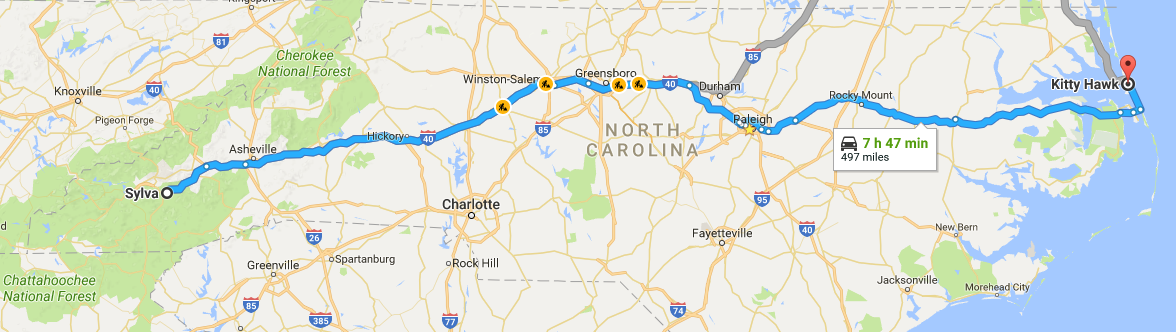
\includegraphics[width=\textwidth]{sylvaKittyHawk_google}
\caption{Google's recommended path from Sylva to Kitty Hawk (497 miles).}
\end{figure}

\begin{figure}[H]
\centering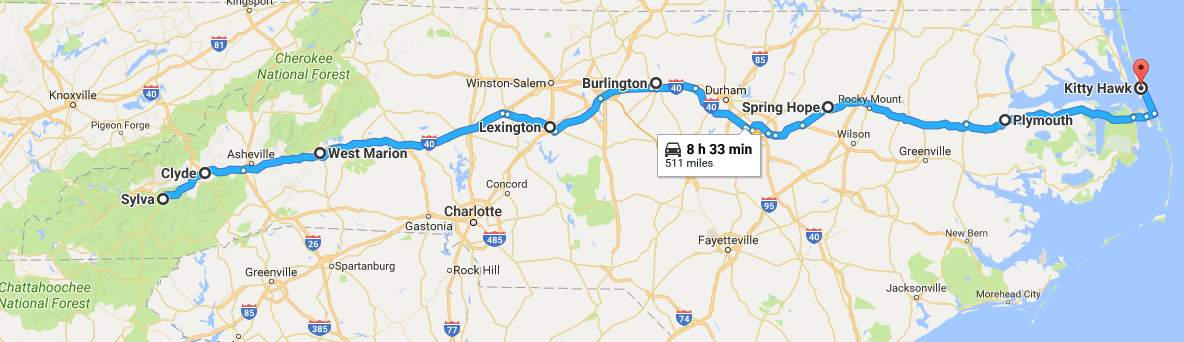
\includegraphics[width=\textwidth]{sylvaKittyHawk_dijkstra511}
\caption{Dijkstra's algorithm's recommended path from Sylva to Kitty Hawk (511 miles).}
\end{figure}

Note that the difference in distance and path is due to the way Google Maps directs you to individual cities. When each hop is plotted, it takes the driver off of the highway, which adds distance that wouldn't be considered if you were driving the whole way without stopping. But generally, the path given by Dijkstra's algorithm does appear similar to Google's. Note that Dijkstra's algorithm is optimizing distance while Google considers time in addition to distance. The next example illustrates this trade-off clearly.

\begin{figure}[H]
\centering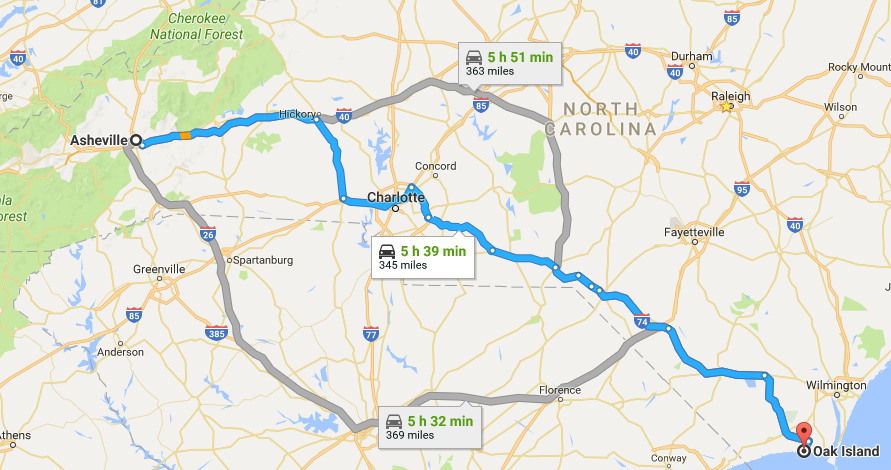
\includegraphics[width=0.7\textwidth]{ashevilleOakIsland_google}
\caption{Google's recommended path from Asheville to Oak Island (345 miles).}
\end{figure}
\begin{figure}[H]
\centering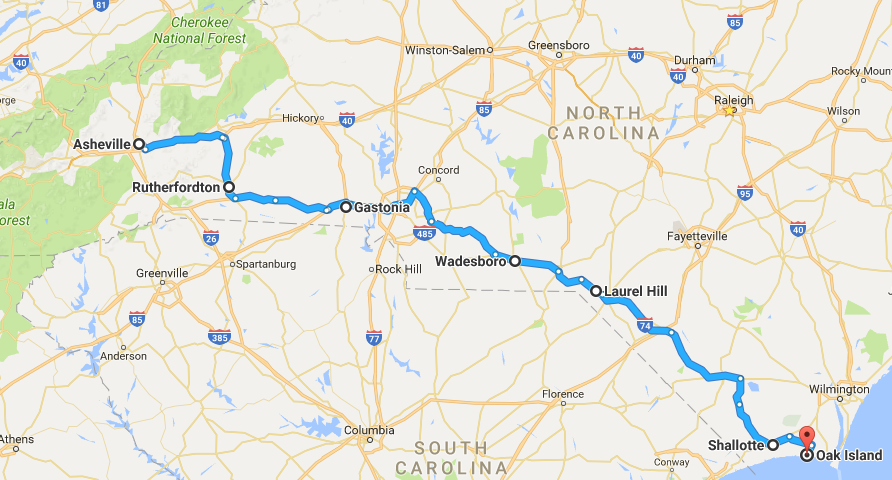
\includegraphics[width=0.7\textwidth]{ashevilleOakIsland_dijkstra349}
\caption{Dijkstra's algorithm's path from Asheville to Oak Island (349 miles).}
\end{figure}

Note that the paths are quite different at first. This can be attributed to the way Google optimizes for distance as well as time. In Google's recommended path, the driver would stay on Interstate 40 for a while before branching down to the Charlotte area. This is primarily to take advantage of the higher speed limits on the highway. Dijkstra's algorithm, only optimizing for distance, shows a higher total distance. This is only because Google Maps can't be finagled into mapping a very direct route without manual interference. So the indirect hop between Asheville and Rutherfordton is still present in the Dijkstra mapping. The table below summarizes these results.

\begin{table}[H]
\centering\makegapedcells
\begin{tabular}{|| c c c c ||}
\hline
\textbf{Start} & \textbf{Finish} & \textbf{Dijkstra (hops)} & \textbf{Google} \\
\hline
Sylva & Kitty Hawk & 511 (10) & 497 \\
Asheville & Oak Island & 349 (8) & 345 \\
\hline
\end{tabular}
\caption{Comparison of the results of Dijkstra's algorithm and Google's recommended path.}
\end{table}

\end{document}